\documentclass[14pt]{extarticle}
\usepackage[a4paper, left=2cm, right=2cm, top=1.5cm, bottom=2cm]{geometry}
\usepackage[utf8]{inputenc}
\usepackage[T2A]{fontenc}
\usepackage[russian]{babel}
\usepackage{indentfirst}
\usepackage{enumitem}
\usepackage{amsmath,amsfonts,amssymb}
\usepackage{icomma}
\usepackage{graphicx}
\usepackage{framed}
\usepackage{caption}
\usepackage{float}
\usepackage{titletoc}
\usepackage{hyperref}
\usepackage{paratype}
\renewcommand{\rmdefault}{PTSans-TLF}


\begin{document}
	
	\thispagestyle{empty}
	
	\begin{center}
		
		\textbf{Санкт-Петербургский политехнический университет}\\
		\vspace{2cm}
		
		Направление подготовки \\
		\large <<01.03.02 Прикладная математика и информатика>>\\
		
		\vspace{7cm}
		
		Отчет по лабораторной работе №7:\\
		\vspace{0.2cm}
		\textbf{\LARGE Решение краевой задачи для ОДУ 2-ого порядка)}
		
		\vspace{6cm}
		
		\begin{flushleft}
			Выполнил студент гр. 5030102/40003 \hfill Т.Р. Абдуллин\\
			Преподаватель: \hfill К.Н. Козлов\\
		\end{flushleft}
		
		\vspace{3cm}
		
		Санкт-Петербург\\
		2026
	\end{center}
	
	%-------- the beginning of report --------
	
	\tableofcontents
	
	%-------- the first point --------
	\newpage
	\section{\Large \underline{Формулировка задачи и ее формализация}}
	\subsection{Формулировка задачи}
	
	Требуется численно решить краевую задачу для обыкновенного
	дифференциального уравнения второго порядка на отрезке $[0, 1]$
	методом факторизации (расщепления).
	
	Исследуемое уравнение имеет вид:
	
	\[
	y'' + (1 + \sin^2 x)y' + (\cos^2 x)y = 3e^x
	\]
	
	Краевые условия:
	
	\[
	\begin{cases}
		y(0) + y'(0) = 2, \\
		y(1) = e
	\end{cases}
	\]
	
	Точное решение задачи:
	
	\[
	y(x) = e^x
	\]
	
	Требуется:
	
	\begin{itemize}
		\item реализовать метод факторизации;
		\item организовать вычисление с фиксированным и адаптивным шагом;
		\item исследовать точность численного метода;
		\item построить графики численного и точного решений;
		\item исследовать зависимость фактической погрешности от заданной точности;
		\item построить график изменения шага по отрезку.
	\end{itemize}
	
	\subsection{Формализация задачи}
	
	Преобразуем исходное уравнение к системе задач Коши методом факторизации.
	
	Ищем функциональную связь в виде:
	
	\[
	y'(x) = \alpha(x) y(x) + \beta(x)
	\]
	
	Дифференцируя и подставляя в исходное уравнение, получаем задачу Коши прямого хода:
	
	\[
	\begin{cases}
		\alpha' = -\alpha^2 - (1 + \sin^2 x)\alpha - \cos^2 x, \\
		\beta' = -(\alpha + 1 + \sin^2 x)\beta + 3e^x
	\end{cases}
	\]
	
	начальные данные:
	
	\[
	\alpha(0) = -1, \qquad \beta(0) = 2
	\]
	
	Граничное условие на правом конце:
	
	\[
	y(1) = e
	\]
	
	Задача Коши обратного хода:
	
	\[
	\begin{cases}
		y' = \alpha(x) y + \beta(x), \\
		y(1) = e
	\end{cases}
	\]
	
	Рассматриваемый отрезок:
	
	\[
	x \in [0, 1]
	\]
	
	%-------- the second point --------
	
	\newpage
	\section{\Large \underline{Алгоритм метода}}
	
	\subsection{Псевдокод метода}
	
	Метод факторизации состоит из прямого хода (решение нелинейной системы ОДУ)
	и обратного хода (решение линейного ОДУ 1-го порядка).
	Интегрирование проводится методом Рунге-Кутты 4-го порядка.
	
	Формулы метода:
	
	\[
	k_1 = f(x_n, Y_n)
	\]
	\[
	k_2 = f\left(x_n + \frac{h}{2}, Y_n + \frac{h}{2} k_1\right)
	\]
	\[
	k_3 = f\left(x_n + \frac{h}{2}, Y_n + \frac{h}{2} k_2\right)
	\]
	\[
	k_4 = f(x_n + h, Y_n + h k_3)
	\]
	\[
	Y_{n+1} = Y_n + \frac{h}{6}(k_1 + 2k_2 + 2k_3 + k_4)
	\]
	
	Критерий адаптивного шага (правило Рунге):
	
	\[
	\delta = \frac{\|Y_{half} - Y_{full}\|}{15} \le \varepsilon
	\]
	
	Псевдокод алгоритма:
	
	\begin{enumerate}
		\item Задать:
		\[
		a = 0,\ b = 1,\ \alpha(0) = -1,\ \beta(0) = 2,\ y(1) = e,\ \varepsilon
		\]
		
		\item Положить:
		\[
		x_0 = a
		\]
		
		\item \textbf{Прямой ход:} пока $x_n < b$ выполнять:
		
		\begin{enumerate}
			\item Вычислить шаг $h$ и оценить ошибку $\delta$.
			\item Если $\delta \le \varepsilon$:
			\begin{itemize}
				\item принять шаг: сохранить $x_{n+1}, \alpha_{n+1}, \beta_{n+1}$ и промежуточные полушаги;
				\item положить $x_n = x_{n+1}$.
			\end{itemize}
			\item Иначе:
			\begin{itemize}
				\item уменьшить шаг $h$;
				\item повторить вычисление.
			\end{itemize}
		\end{enumerate}
		
		\item Задать граничное значение на правом конце:
		\[
		y(b) = e
		\]
		
		\item \textbf{Обратный ход:} для каждого узла от $x = b$ до $x = a$ выполнять:
		
		\begin{enumerate}
			\item Сделать шаг назад по сохраненным значениям $\alpha$ и $\beta$:
			\[
			y' = \alpha(x) y + \beta(x)
			\]
			\item Сохранить $y(x_n)$.
		\end{enumerate}
	\end{enumerate}
	
	\subsection{Условия применимости метода}
	
	Для применимости метода факторизации необходимо выполнение следующих условий:
	
	\begin{enumerate}
		\item Коэффициенты $p(x), q(x), r(x)$ и $f(x)$ должны быть непрерывны, при этом $p(x) \ne 0$.
		\item Решение уравнения Риккати $\alpha(x)$ должно быть ограничено на $[a, b]$ (отсутствие полюсов).
		\item Знаменатель граничного соотношения на правом конце должен быть отличен от нуля:
		\[
		\beta_0 + \beta_1 \alpha(b) \ne 0
		\]
		\item Шаг интегрирования должен обеспечивать численную устойчивость.
	\end{enumerate}
	
	%-------- the third point --------
	
	\newpage
	\section{\Large \underline{Проверка условий применимости}}
	
	\begin{figure}[H]
		\centering
		\begin{framed}
			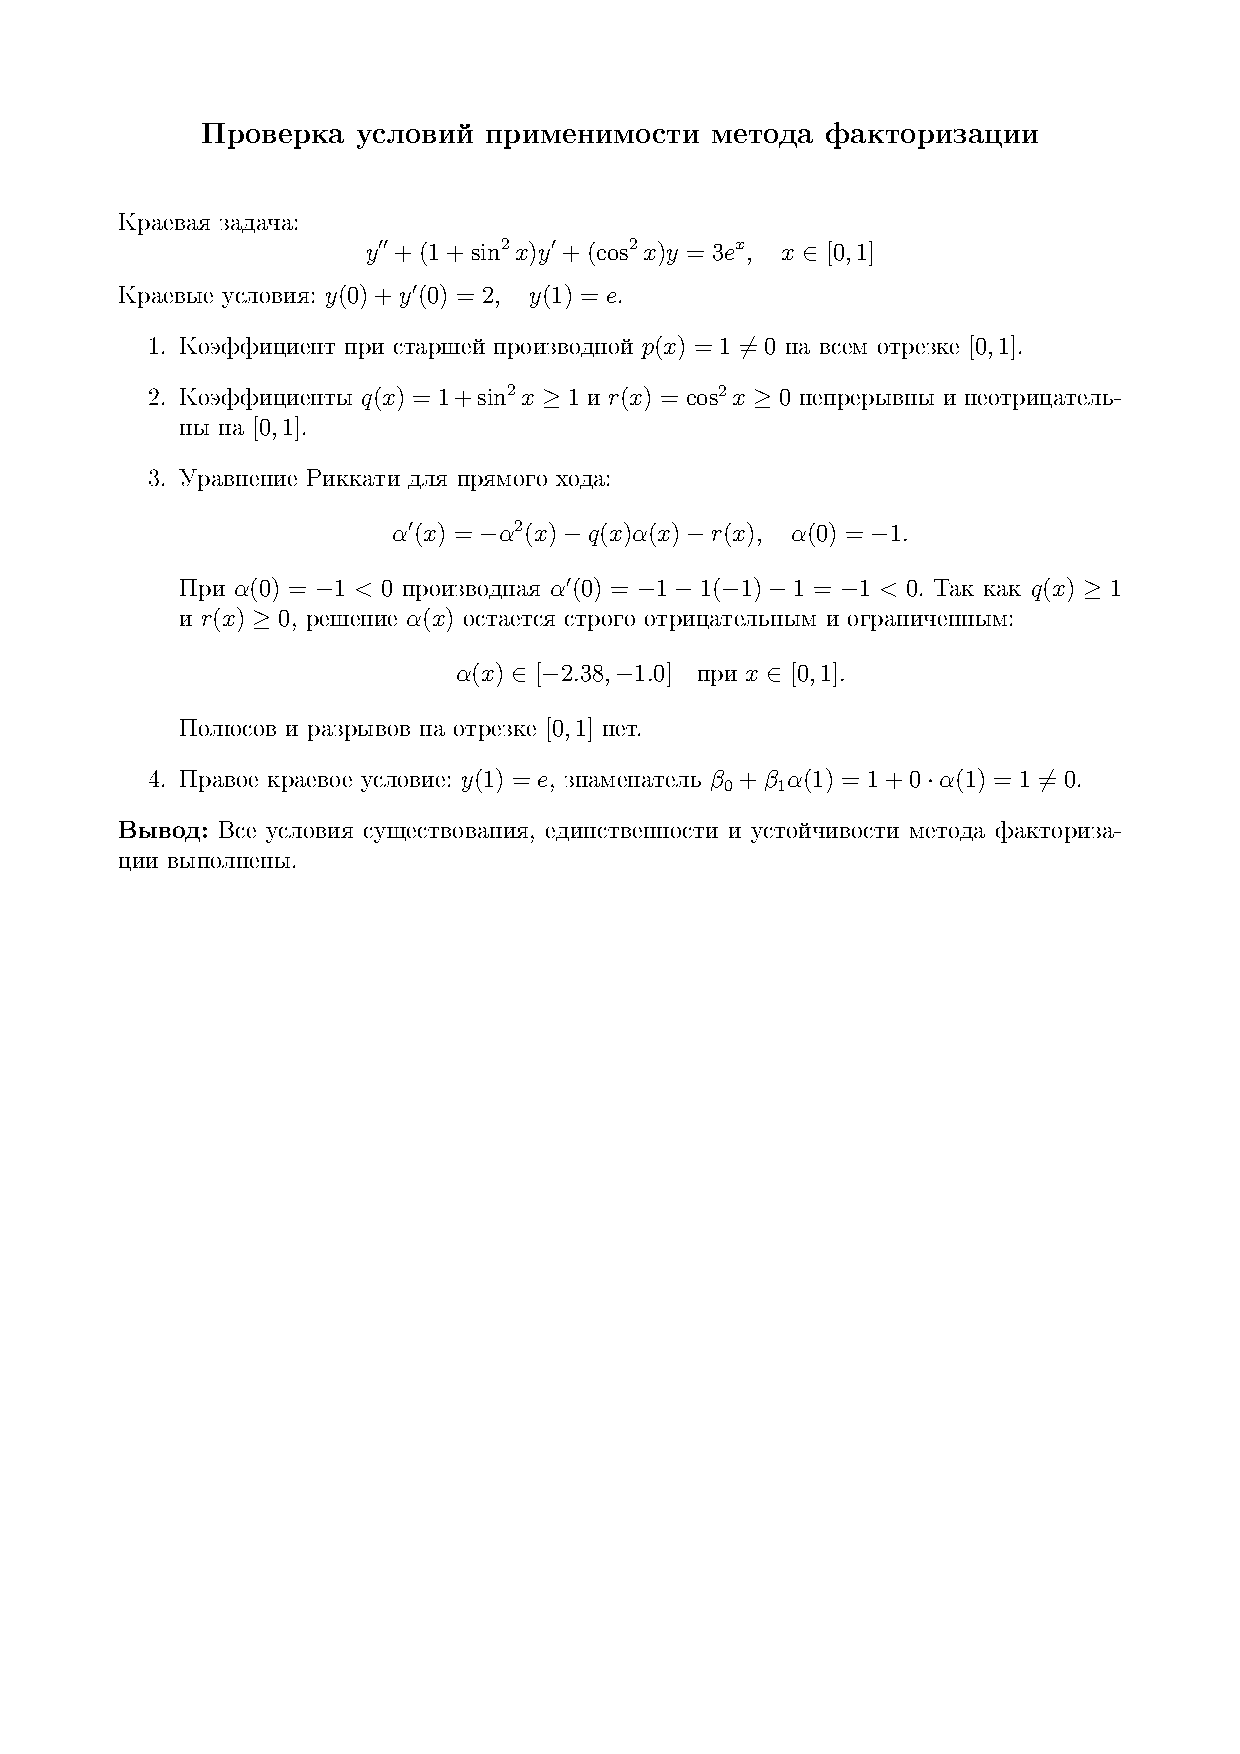
\includegraphics[width=0.9\linewidth]{../data/check.pdf}
			\caption{Проверка условий применимости}
			\label{fig:check}
		\end{framed}
	\end{figure}
	
	%-------- the fourth point --------
	
	\newpage
	\section{\Large \underline{Тестовый пример}}
	
	\begin{figure}[H]
		\centering
		\begin{framed}
			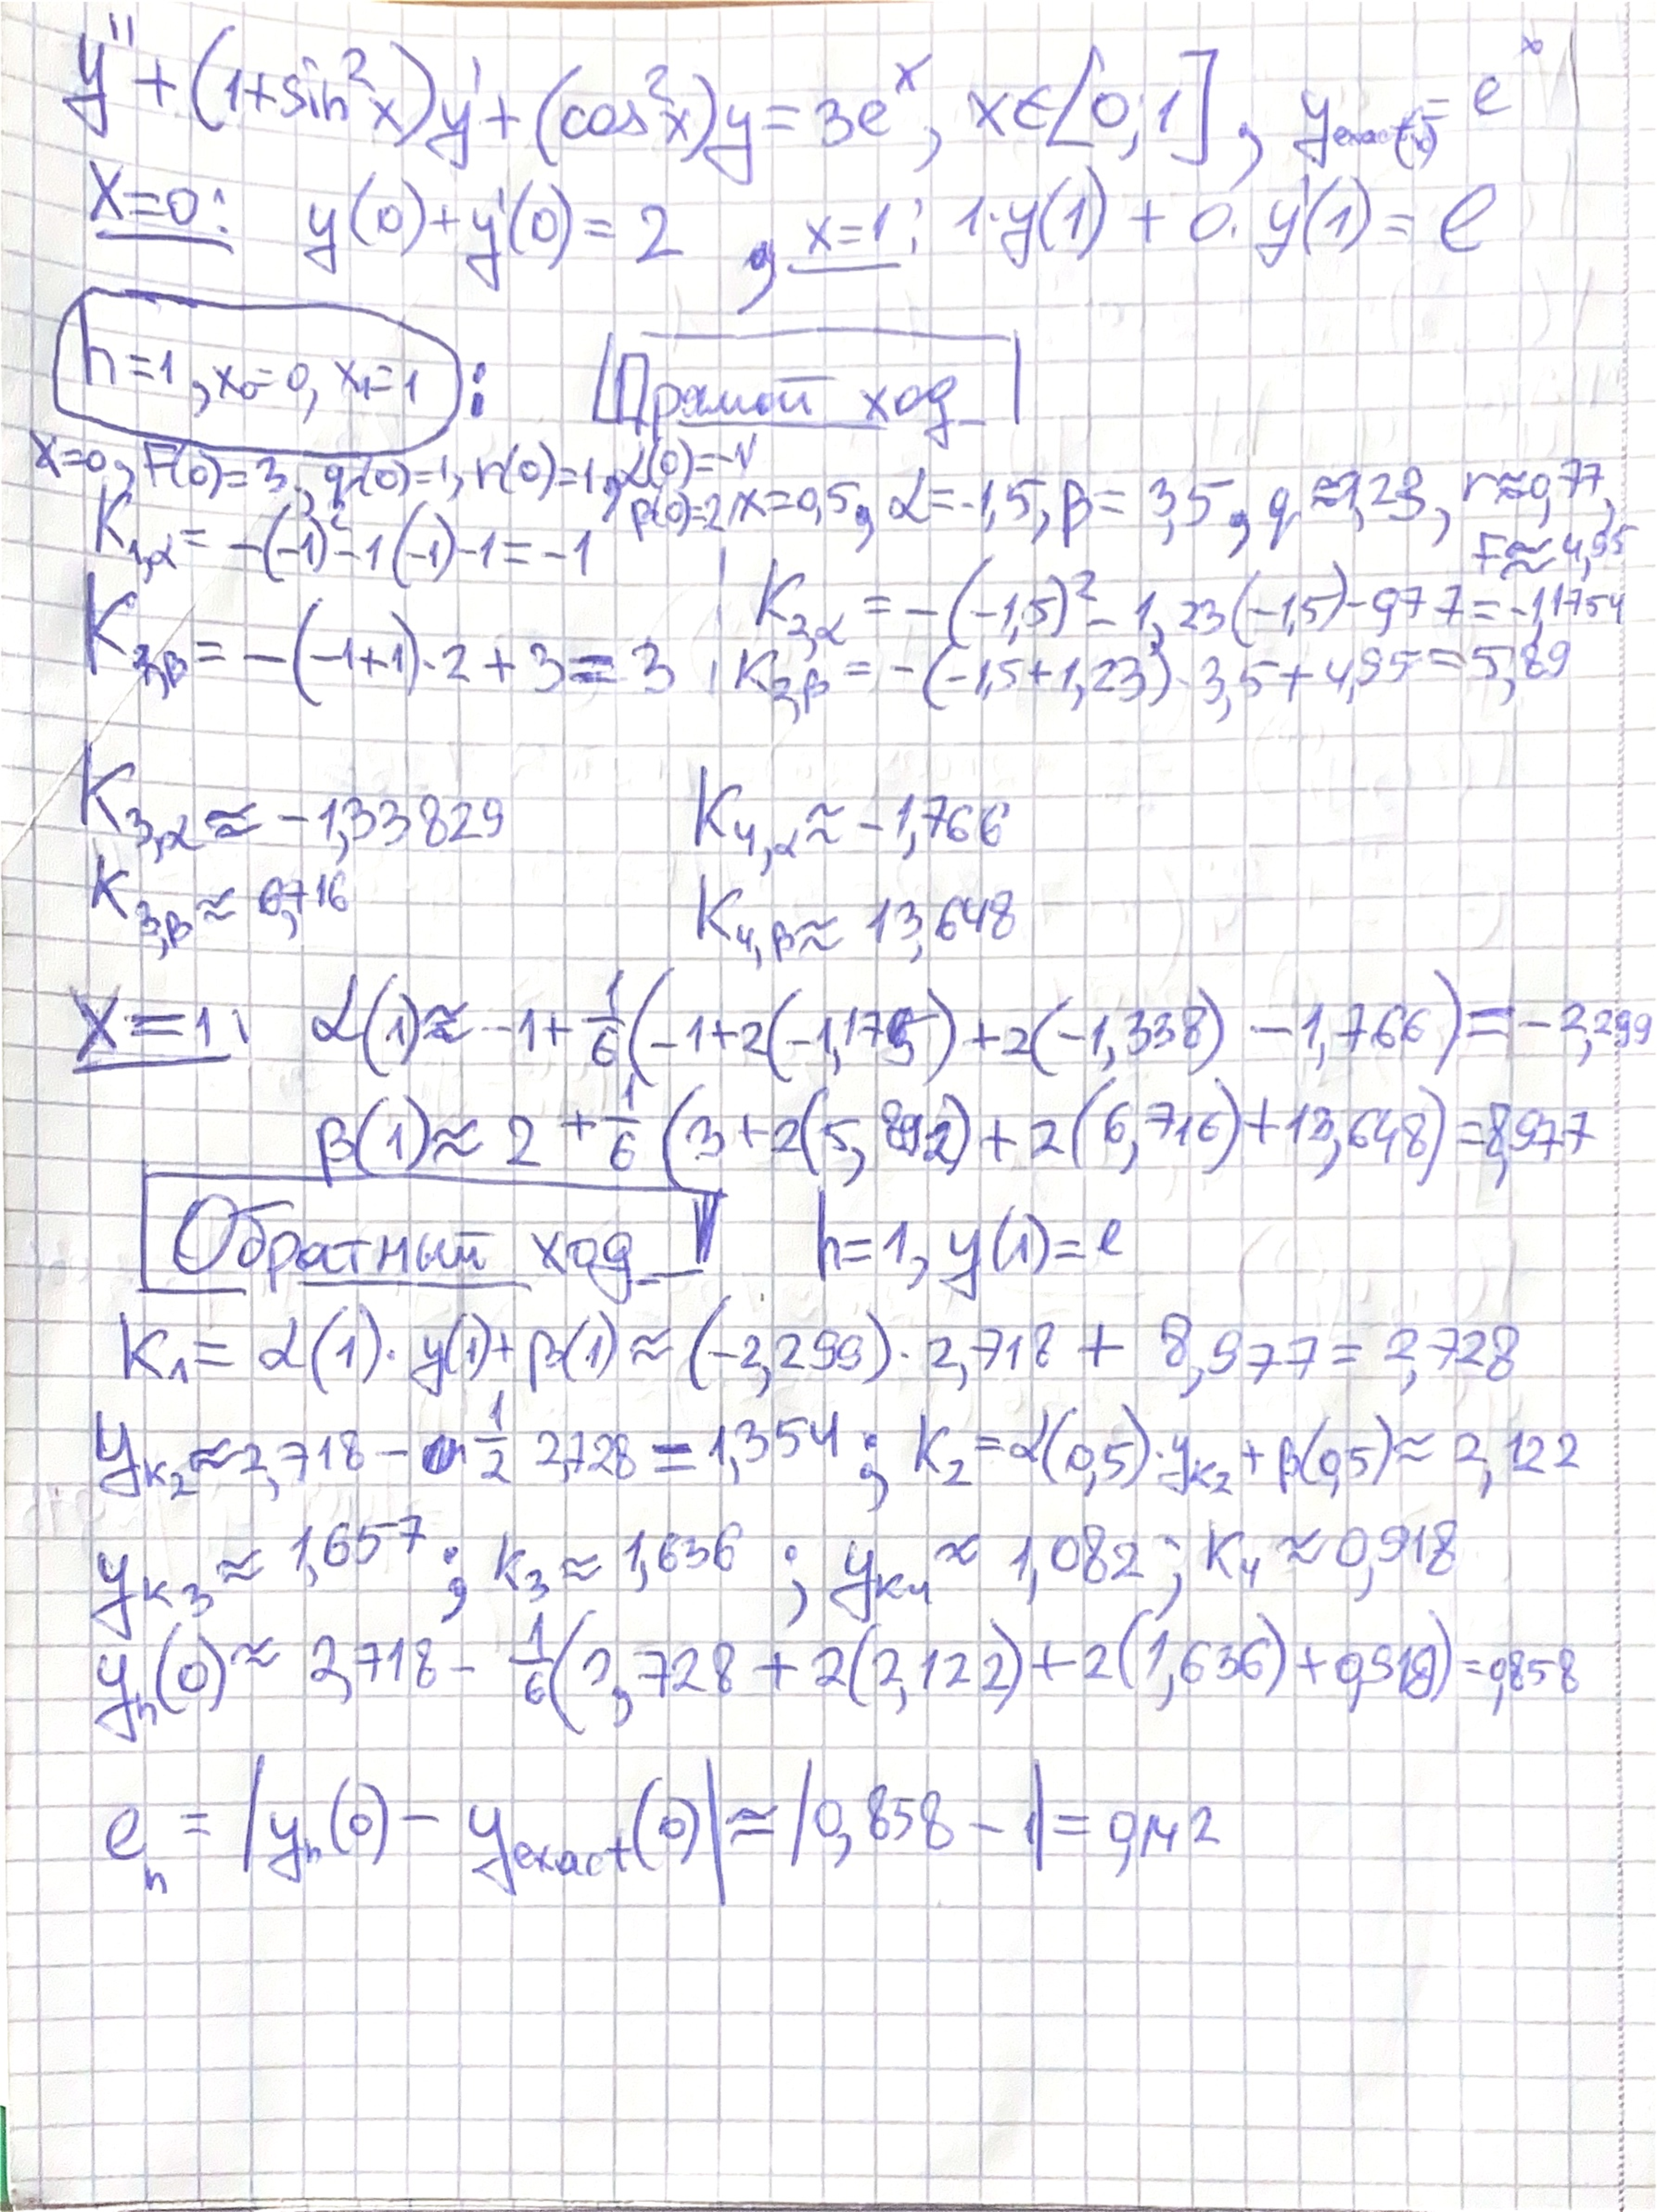
\includegraphics[width=0.9\linewidth]{../data/test_example.pdf}
			\caption{Тестовый пример (1)}
			\label{fig:test_1}
		\end{framed}
	\end{figure}
	
	\begin{figure}[H]
		\centering
		\begin{framed}
			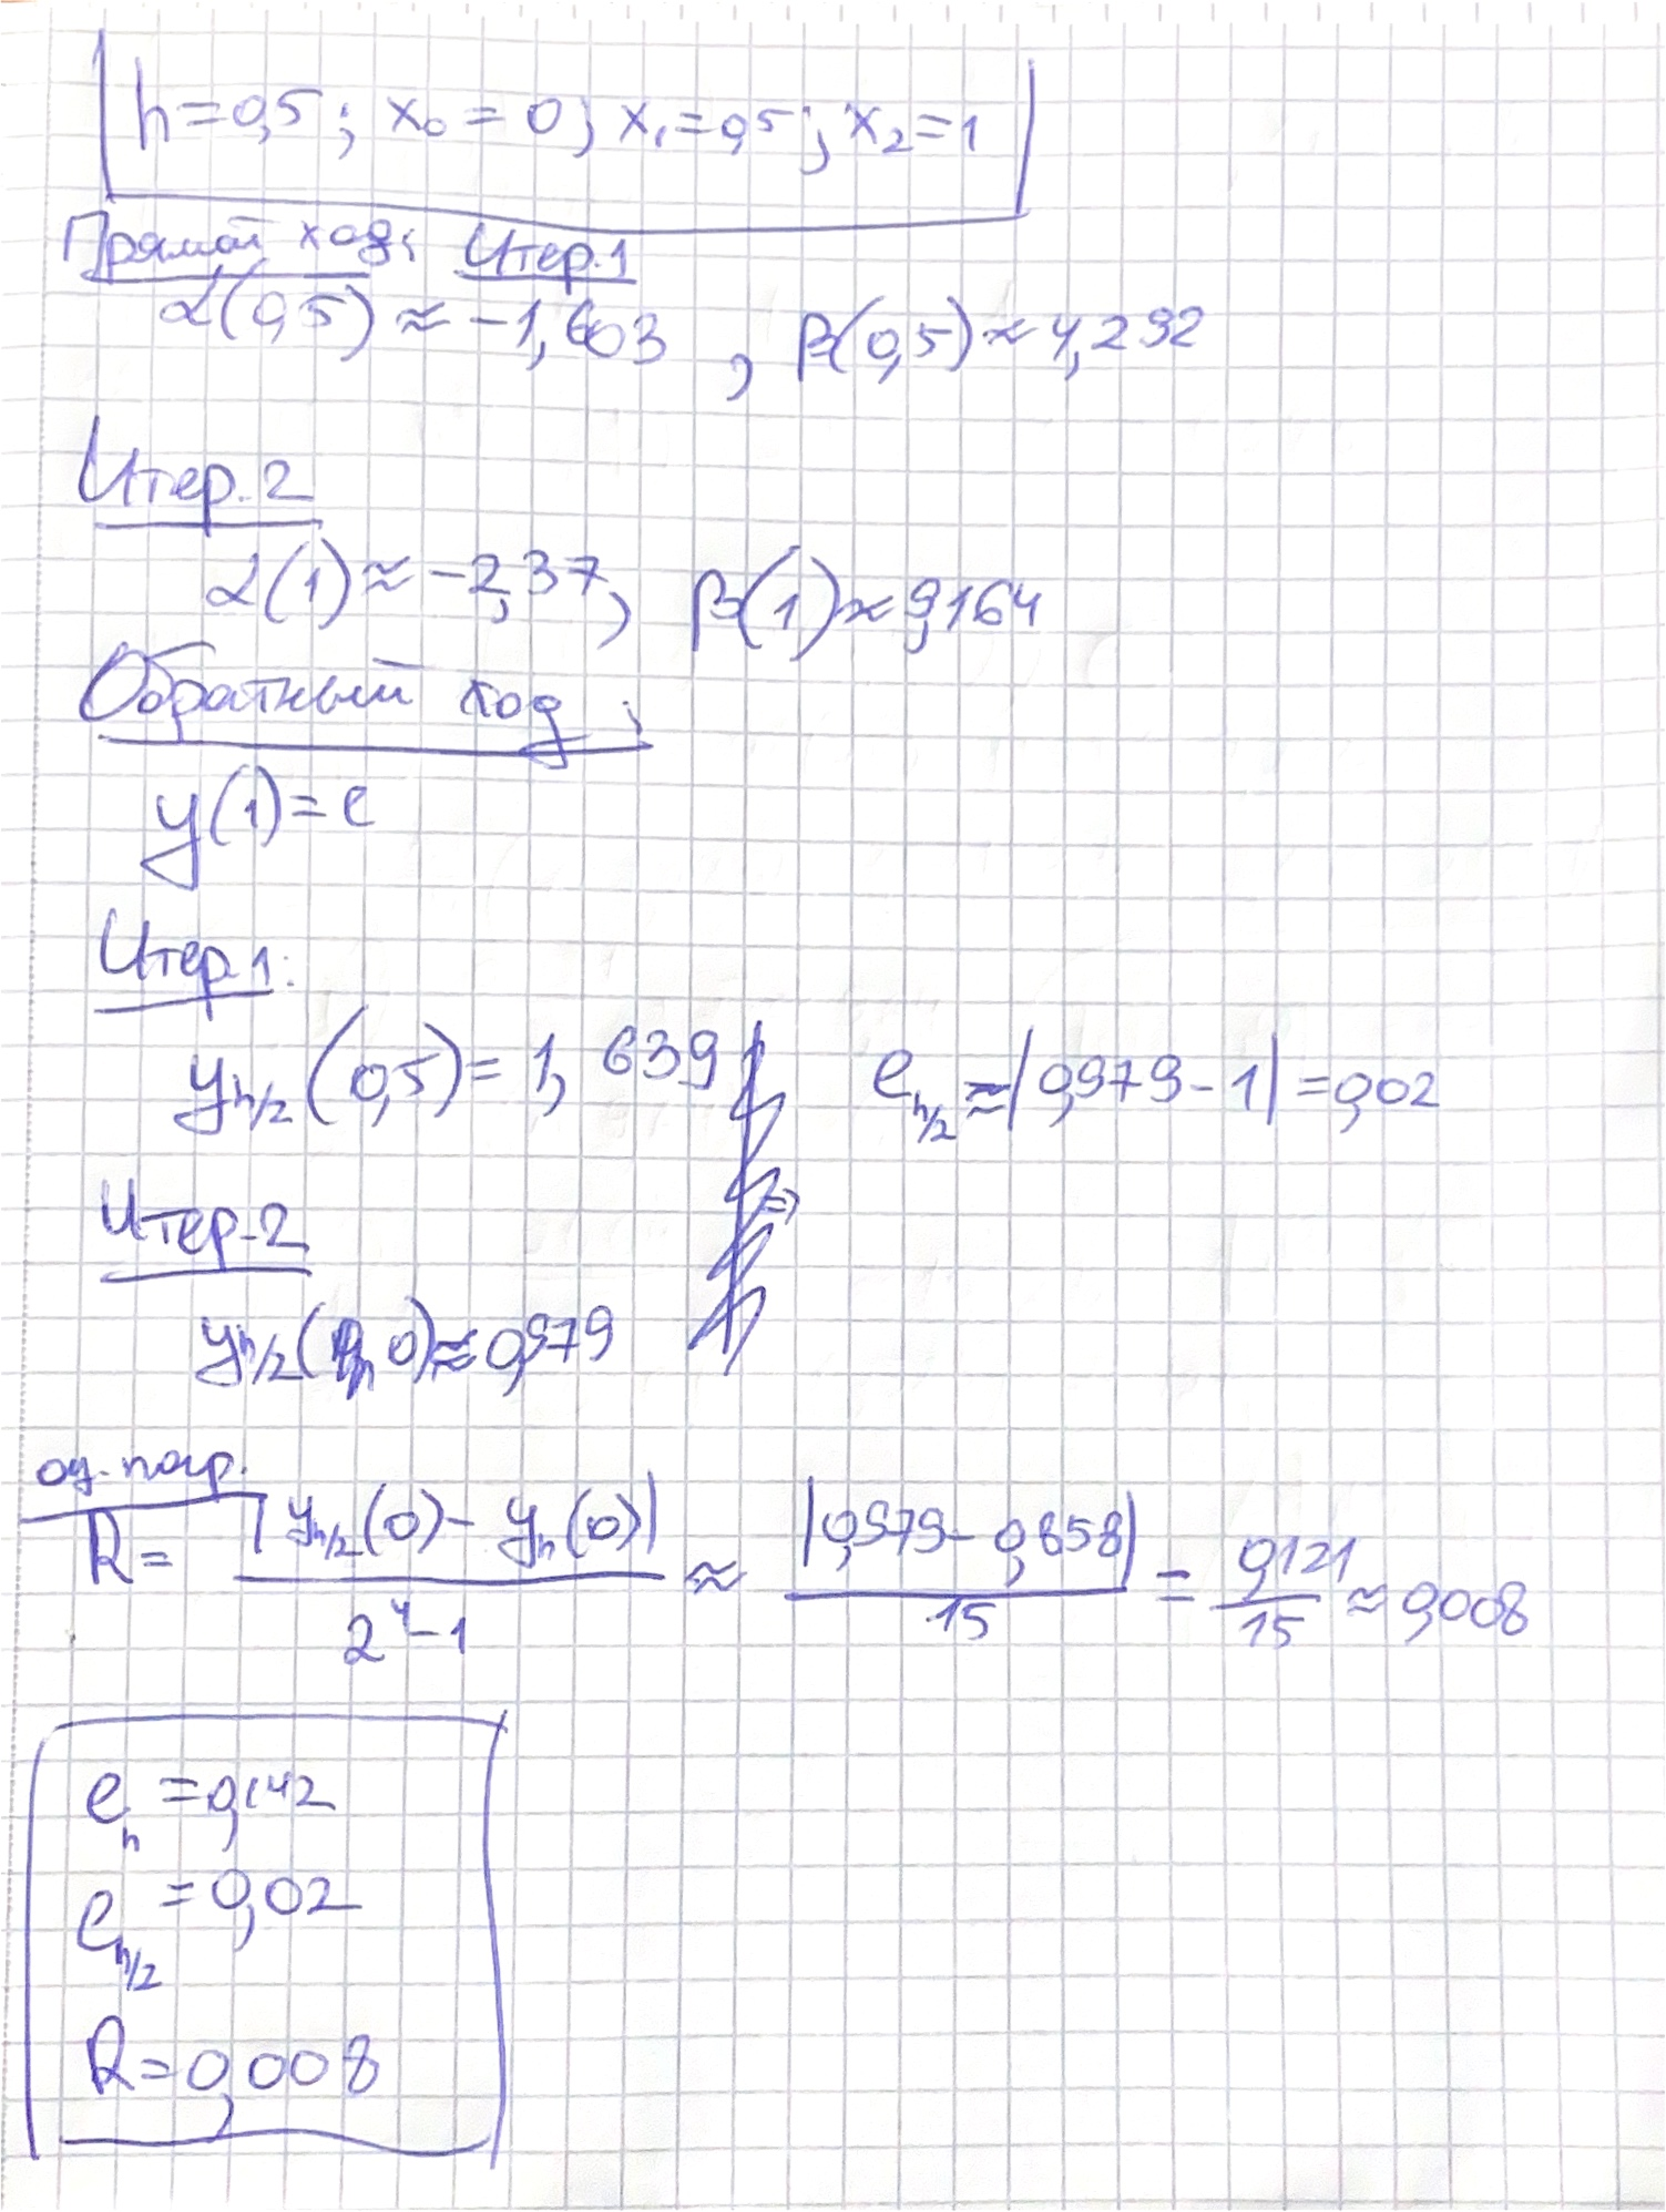
\includegraphics[width=0.9\linewidth]{../data/test_example_2.pdf}
			\caption{Тестовый пример (2)}
			\label{fig:test_2}
		\end{framed}
	\end{figure}
	
	Видно, что при уменьшении шага в 2 раза погрешность численного решения методом Рунге-Кутты уменьшается практически на порядок (с $0.142$ до $0.021$), а оценка по правилу Рунге ($R = 8.07 \times 10^{-3}$) хорошо согласуется с фактическим снижением погрешности.
	
	%-------- the fifth point --------
	
	\newpage
	\section{\Large \underline{Подготовка контрольных тестов}}
	
	Для проверки корректности реализации используется задача,
	имеющая известное аналитическое решение.
	
	Исследуемая задача:
	
	\[
	y'' + (1 + \sin^2 x)y' + (\cos^2 x)y = 3e^x
	\]
	
	Краевые условия:
	
	\[
	y(0) + y'(0) = 2, \qquad y(1) = e
	\]
	
	Точное решение:
	
	\[
	y(x) = e^x
	\]
	
	Контроль осуществляется следующим образом:
	
	\begin{enumerate}
		\item Вычисляется численное решение.
		\item В узлах сетки вычисляется точное решение.
		\item Определяется абсолютная погрешность:
		
		\[
		e_i = |y_i^{num} - y_i^{exact}|
		\]
		
		\item Определяется максимальная ошибка:
		
		\[
		E = \max_i e_i
		\]
	\end{enumerate}
	
	Для исследования метода используются:
	
	\begin{itemize}
		\item различные шаги интегрирования;
		\item различные значения заданной точности;
		\item исследование изменения шага по отрезку.
	\end{itemize}
	
	%-------- the sixth point --------
	
	\section{\Large \underline{Модульная структура программы}}
	
	\begin{itemize}
		\item \textbf{q\_func, r\_func, f\_func} — вычисление коэффициентов уравнения
		\begin{itemize}
			\item вход: $x$
			\item выход: значение коэффициента.
		\end{itemize}
		
		\item \textbf{factorization\_fixed} — метод факторизации с фиксированным шагом
		\begin{itemize}
			\item вход: $a, b, h$
			\item выход: вектор точек решения.
		\end{itemize}
		
		\item \textbf{factorization\_adaptive} — метод факторизации с адаптивным шагом
		\begin{itemize}
			\item вход: $a, b, \varepsilon$
			\item выход: вектор точек решения и история шагов.
		\end{itemize}
	\end{itemize}
	
	%-------- the eighth point --------
	
	\newpage
	\section{\Large \underline{Численный анализ решения задачи}}
	
	\begin{enumerate}[label*=\arabic*), align=left, leftmargin=*, itemindent=1.5em, listparindent=1.5em, parsep=0pt]
		\begin{figure}[H]
			\centering
			\begin{framed}
				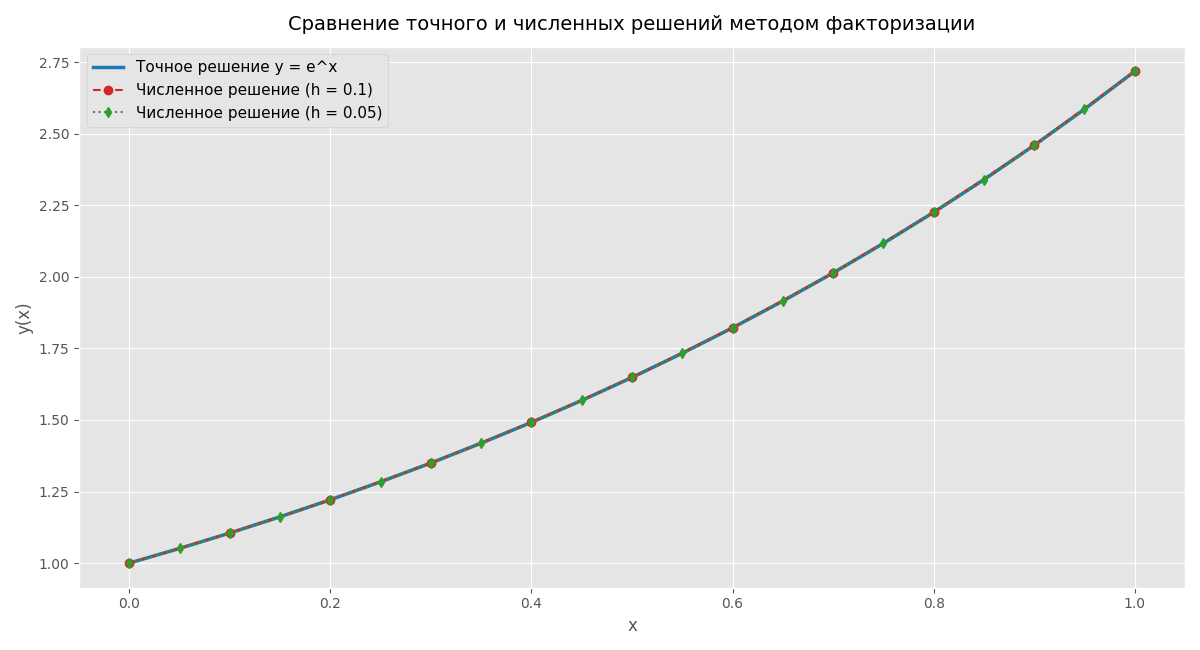
\includegraphics[width=0.9\linewidth]{../data/solves.png}
				\caption{График точного решения и решения метода}
				\label{fig:solves}
			\end{framed}
		\end{figure}
		
		\begin{figure}[H]
			\centering
			\begin{framed}
				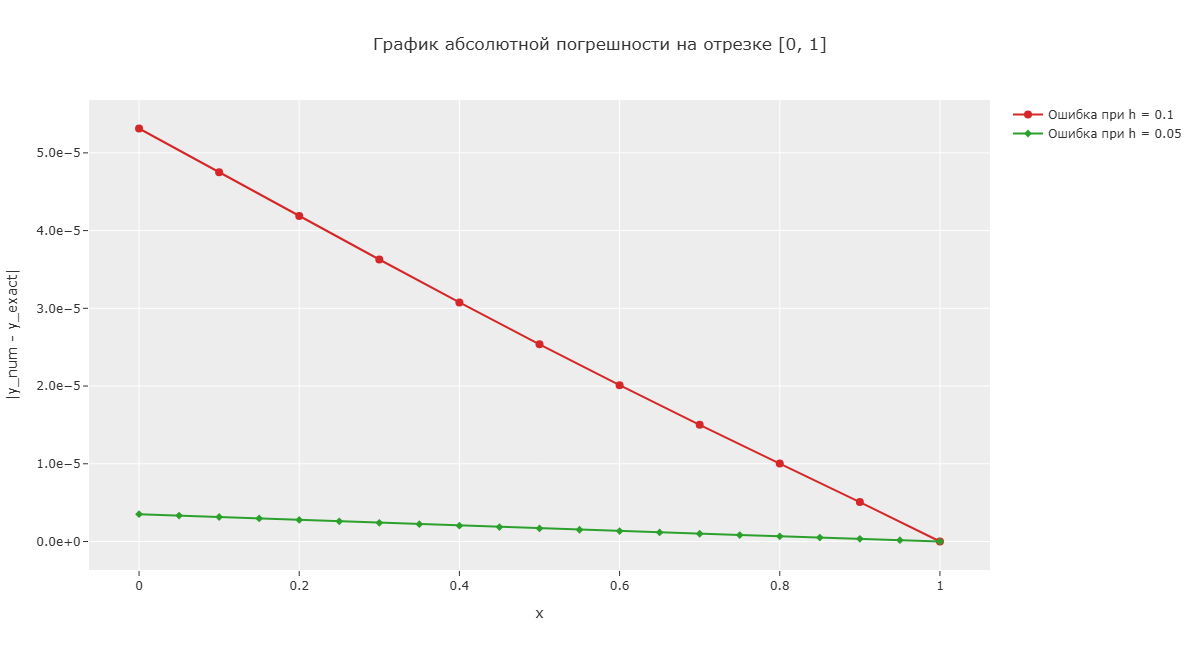
\includegraphics[width=0.9\linewidth]{../data/error.png}
				\caption{График ошибки}
				\label{fig:error}
			\end{framed}
		\end{figure}
		
		\begin{figure}[H]
			\centering
			\begin{framed}
				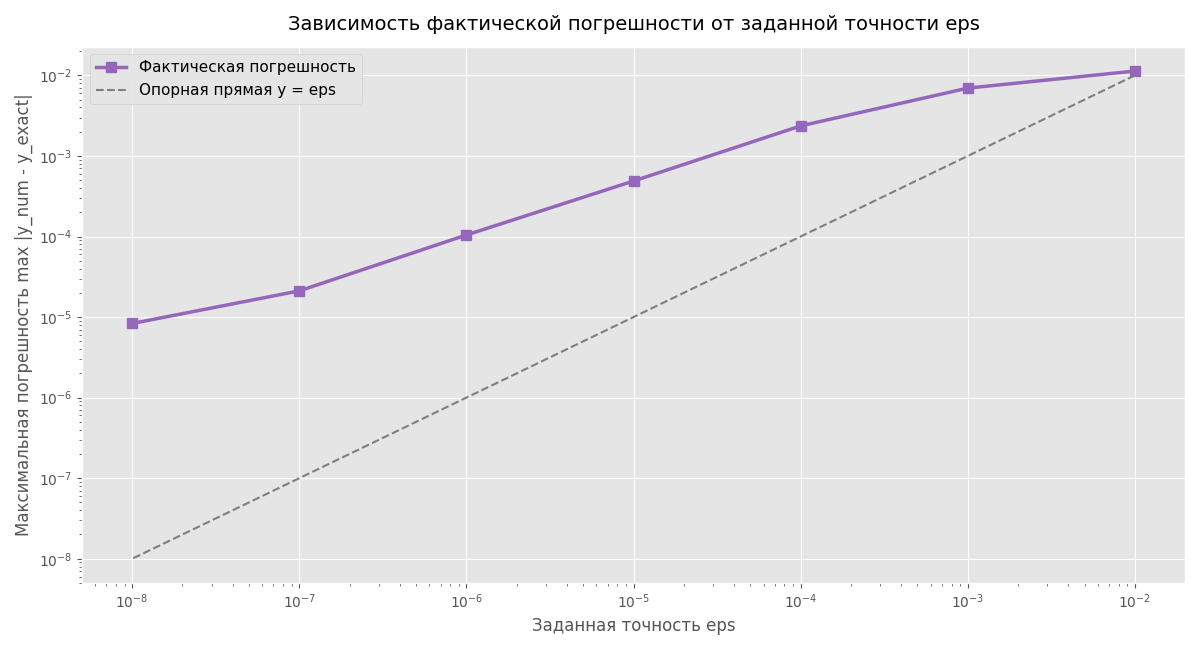
\includegraphics[width=0.9\linewidth]{../data/accuracy.png}
				\caption{График зависимости фактической ошибки от заданной точности}
				\label{fig:accuracy}
			\end{framed}
		\end{figure}
		
		\begin{figure}[H]
			\centering
			\begin{framed}
				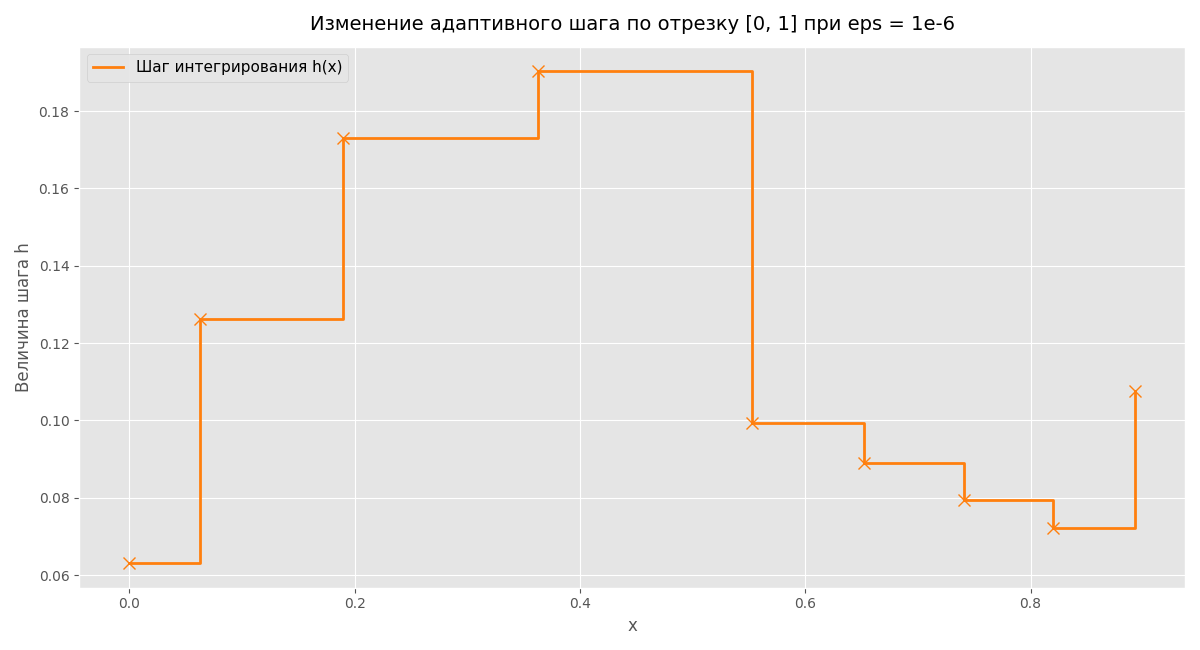
\includegraphics[width=0.9\linewidth]{../data/step_size.png}
				\caption{График изменения шага по отрезку}
				\label{fig:step}
			\end{framed}
		\end{figure}
		
		\newpage
		\item Построен график решений: точного и метода \eqref{fig:solves}.
		
		Решение метода визуально совпадает с точным.
		
		\item Далее был построен график зависимости ошибки \eqref{fig:error}.
		
		Здесь уже можно пронаблюдать при каких значениях мы получаем соответствующую ошибку. При уменьшении шага в 2 раза ошибка падает примерно в 16 раз, подтверждая 4-й порядок метода.
		
		\item И наконец был построен график зависимости ошибки от заданной точности \eqref{fig:accuracy}.
		
		Чем меньше точность, тем меньше ошибка.
		
		\item Также был построен график изменения адаптивного шага по отрезку \eqref{fig:step}.
		
		В начале отрезка шаг крупнее, а к правому краю измельчается из-за более быстрого роста экспоненты.
		
	\end{enumerate}
	
	%-------- the ninth point --------
	
	\newpage
	\section{\Large \underline{Выводы}}
	
	В ходе лабораторной работы был реализован
	метод факторизации (расщепления)
	для решения краевой задачи
	для обыкновенного дифференциального уравнения
	второго порядка.
	
	В ходе вычислительных экспериментов установлено:
	
	\begin{itemize}
		\item численное решение хорошо совпадает
		с аналитическим;
		\item метод является устойчивым
		на рассматриваемом интервале;
		\item уменьшение заданной точности
		снижает ошибку;
		\item алгоритм адаптивного шага автоматически
		подбирает шаг в зависимости от поведения функций.
	\end{itemize}
	
	Полученные результаты подтверждают
	корректность реализации метода
	и соответствуют теоретическим свойствам
	метода факторизации.
	
\end{document}
